\subsection{Momentum method}
The momentum approach is a technique that accelerates the gradient descent accumulating a velocity vector in directions of persistent reduction \cite{momentum}.

We can define \textit{Classical Momentum} (CM) as:
\begin{align}
    & v_{t+1} = \mu v_t - \epsilon \nabla f(\Theta_t) \\
    & \Theta_{t+1} = \Theta_t + v_{t+1}
\end{align}
where $\epsilon > 0$ is the learning rate, $\mu \in [0,1)$ is the momentum coefficient and $\nabla f(\Theta_t)$ is the gradient at $\Theta_t$. The hyperparameter of momentum determines how quickly the contributions of previous gradients exponentially decay.  Another important aspect is that the larger $\mu$ is, relative to $\epsilon$, the more previous gradients affect the current direction. At the moment, no prior choices of the momentum coefficient and learning rate can be done, these will be studied more in the detail in a later phase of the project where we implement and test these models, but as suggested by \parencite[Chap. 8]{bengio}, common values for $\mu$ are $0.5, 0.9, 0.99$.

The next algorithm is the pseudocode relative to the \textit{Gradient descent with momentum}, given the learning rate and the momentum coefficient, performs a descent approach until termination conditions are met.
\begin{algorithm}[H]
	\caption{Gradient descent with momentum. Termination conditions, learning rate and momentum coefficients have to be determined by testing as it will be shown in a later phase of the project. For the moment we assume that they are given.}
	\label{alg:gdmom}
	\begin{algorithmic}[1]
		\State Initialize $\mathit{\Theta}$ and $\mathbf{v}$
		\While{$termination\ conditions\ not\ met$}
		\State Sample $m$ examples $(x_1,y_1), (x_2,y_2) \dots (x_m,y_m)$
		\State $\mathit{\Tilde{\Theta}} \leftarrow \mathit{\Theta}$
		\If {$Nesterov$}
		\State $\mathit{\Tilde{\Theta}} \leftarrow \mathit{\Tilde{\Theta}} + \mu \mathbf{v}$
		\EndIf
		\State Compute gradient estimate: $\mathbf{g} \leftarrow \frac{1}{m}\nabla_{\mathit{\Tilde{\Theta}}}\sum_i(L(f(x_i,\mathit{\Tilde{\Theta}}),y_i))$
		\State Compute velocity update: $\mathbf{v} \leftarrow \mu \mathbf{v} - \epsilon g$
		\State Apply update: $\mathit{\Theta} \leftarrow \mathit{\Theta} + \mathbf{v}$
		\EndWhile
	\end{algorithmic}
\end{algorithm}
In \hyperref[alg:gdmom]{Algorithm \ref{alg:gdmom}} the amount of samples taken at \textit{line 3} determines the type of \textit{Gradient descent algorithm}, such as:
\begin{itemize}
    \item $\mathbf{m = 1}$: \textit{stochastic gradient descent (SGD)};
    \item $\mathbf{m < n}$, where n is the total number of examples: \textit{batch stochastic gradient descent};
    \item $\mathbf{m = n}$: \textit{standard gradient descent (GD)}.
\end{itemize}
A further improvement is given by a modification of the \textit{CM} approach, called \textit{Nesterov's Accelerated Gradient} (NAG) that, seen as a momentum approach, can be defined as:
\begin{align}
    \label{eq:nag}
    & v_{t+1} = \mu v_t - \epsilon\nabla f(\mathit{\Theta_t} + \mu v_t) \\ 
    & \mathit{\Theta_{t+1} = \mathit{\Theta_t} + v_{t+1}}
\end{align}
The only difference from \textit{CM }is relative to the point where the gradient is computed, in fact NAG performs a partial update to $\mathit{\Theta_t}$ and uses this update to compute the gradient at step $\mathit{t}$. After computing the gradient, the update rule is the same, but in this way NAG allow changing $v$ in a more responsive way. This modification is implemented in \hyperref[alg:gdmom]{Algorithm \ref{alg:gdmom}} at \textit{line 6} where an update to the point of evaluation of the gradient is performed. Differences between \textit{CM} and \textit{NAG} can be seen in \hyperref[fig:NAGvsCM]{\textbf{Figure \ref{fig:NAGvsCM}}}.
\begin{figure}[H]
	\centering
	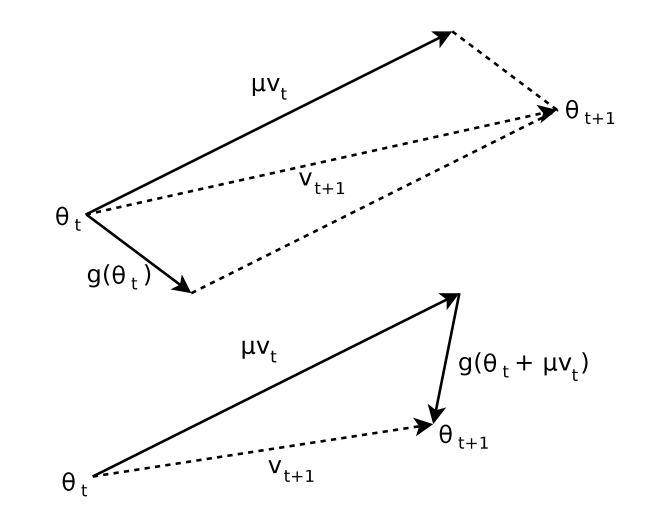
\includegraphics[width=0.4\linewidth]{res/CMvsNAG.png}
	\caption{\textit{\textit{CM} (on top) shows how the update of the vector $v_t$ using the gradient at $\Theta_t$ differs from the \textit{NAG} (on bottom). When $\mu v_t$ is a poor update, we can see how \textit{NAG} points $v_{t+1}$ back towards $\Theta_t$ more strongly than \textit{CM}.}}
	\label{fig:NAGvsCM}
\end{figure}

\subsubsection{Convergence}
\label{conv_mom}
As shown in \cite{momentum}, \textit{NAG} can help avoiding oscillations in the path taken by \textit{CM}. In \hyperref[fig:convNAGvsCM]{\textbf{Figure \ref{fig:convNAGvsCM}}} we can see the comparison between the two momentum methods with same momentum and learning rate coefficients. This shows how the correction rule for a poor update, as shown in \hyperref[eq:nag]{Equation \ref{eq:nag}}, over multiple iterations, can help \textit{NAG} to be more effective than \textit{CM} at decelerating over time. This also helps \textit{NAG} to be more tolerant to larger values of $\mu$ compared to \textit{CM}.
\begin{figure}[H]
	\centering
	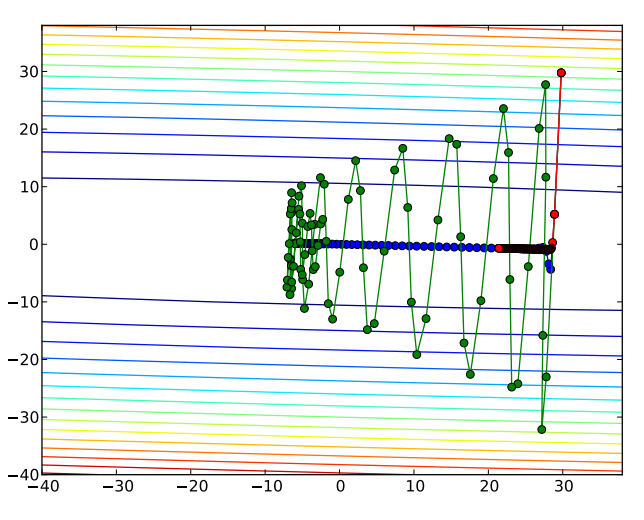
\includegraphics[width=0.35\linewidth]{res/convNAGvsCM.png}
	\caption{\textit{Given the global minimizer of the objective function in (0,0), the red, blue and green curves show, respectively, the trajectories of \textit{gradient descent}, \textit{NAG} and \textit{CM}. It's clearly visible the difference in oscillations between \textit{CM} and \textit{NAG} approach.}}
	\label{fig:convNAGvsCM}
\end{figure}
To study convergence of the \textit{SGD} involving \textit{CM} and \textit{NAG}, applied to a non-convex objective function, we refer to the results obtained in \cite{sgdunified} that describes a unified framework for both momentum methods. The unified framework uses the constant $s=0$ and $s=1$ to refer, respectively, to \textit{CM} and \textit{NAG}. By defining $C>0$ a positive constant and $\mathit{G}_k = \mathit{G}(x_k; \xi_k)$ a stochastic gradient  of $f(x)$ at $x_k$, depending on a random variable $\xi_k$, such that ${\mathbb{E}[\mathit{G}(x_k;\xi_k)] = \nabla f(x_k)}$, the following theorem shows the convergence of \textit{SGD} with momentum for a non-convex objective function $f(x)$.
\begin{thm}
\label{thm:convmom}
Suppose $f(x)$ is a non-convex and L-smooth function, ${\mathbb{E}[\norm{\mathit{G}(x;\xi)-\nabla f(x)}^2]\leq\delta^2}$ and $\norm{\nabla f(x)}\leq\mathit{B}$ for any $x$. Let the stochastic gradient descent method run for $t$ iterations.\\By setting $\epsilon = \min\{\frac{1-\mu}{2L[1+((1-\mu)s-1)^2]}\,,\frac{C}{\sqrt{t+1}}\}$ we have:
\begin{align*}
    \min_{k=0,...,t}\mathbb{E}[\norm{\nabla f(x_k)}^2] &\leq \frac{2(f(x_0)-f^*)(1-\mu)}{t+1}\max\Big\{\frac{2L[1+((1-\mu)s-1)^2]}{1-\mu}\,,\frac{\sqrt{t+1}}{C}\Big\}\\
    &+\frac{C}{\sqrt{t+1}}\frac{L\mu^2(\mathit{B}^2+\delta^2)+L\delta^2(1-\mu)^2}{(1-\mu)^3}
\end{align*}
\end{thm}
This theorem shows that the gradient norm converges in expectation at $\mathcal{O}(\frac{1}{\sqrt{t}})$ \cite{sgdunified}.
Additionally, \textbf{Theorem \ref{thm:convmom}} suggests that for \textit{NAG} ($s=1$) we can set a larger initial learning rate than that of \textit{CM} ($s=0$), as also shown in \parencite[Section 4]{sgdunified}, which leads to a faster convergence in training error.

However, noting that in our case the assumptions made for \textbf{Theorem \ref{thm:convmom}} do not hold, in particular our objective function is not continuously differentiable and not Lipschitz continuous, we can't use this result to prove convergence for our setting. At the moment we are not able to state anything about the converge, in practice, of our algorithm with our specific setting (i.e. non-convex, non-differentiable objective function), so we postpone this discussion in the testing phase.
% It is worthwhile to note that a sufficient condition to guarantee \textit{SGD} convergence in practice is, as stated in \text{{\parencite[Chap. 8]{bengio}}}:
% \begin{align*}
%     \sum_{k=1}^\infty\epsilon_k=\infty\, \, and\, \, \sum_{k=1}^\infty\epsilon_k^2<\infty \text{ with $\epsilon_k$ learning rate at step $k$.}
% \end{align*}